\section{Solid 2 - OCP, LSP og DIP}

\subsection{Fokuspunkter}

\begin{itemize}
	\item Redegør for:
	\begin{itemize}
		\item Open-Closed Principle (OCP).
		\item Lisskov's Substitution Principle (LSP).
		\item Dependency Inversion Principle (DIP).
	\end{itemize}
	\item Redegør for, hvordan du mener anvendelsen af principperne fremmer godt SW design.
	\item Vis et eksempel på anvendelsen af et eller flere af principperne i SW design.
	\item Redegør for konsekvenserne ved anvendelsen af OCP, LSP og/eller DIP - har det nogle ulemper?
\end{itemize}

\subsection{Open-Closed Principle (OCP)}\label{sec:ocp}
\textit{''Open for extension, closed for modification''}\\

OCP siger at man bør refaktorere således at yderligere ændringer ikke skaber problemer\footnote{rekompilering, retest, redeploy.} i resten af programmet.\\

Når OCP er "well applied" betyder det at vi kan tilføje ny kode uden at behøve ændre i eksisterende kode, som er testet og virker.

\paragraph{De 2 primære attributter:}
\begin{enumerate}
	\item Open for extension - Modulet kan udvides i takt med at krav udvides.
	\item Closed for modification - Ved kun at udvide programmet, behøves vi ikka at røre ved exekverbare filer, DLL'er og library filer.
\end{enumerate}

\subsubsection{HOW TO OCP}

\begin{itemize}
	\item Brug abstrakte klasser, som base.
	\item Eksempel - Client der bruger Server.
	\item To konkrete klasser er lort $\longrightarrow$ brug et interface.
\end{itemize}

\begin{figure}[H]
\centering
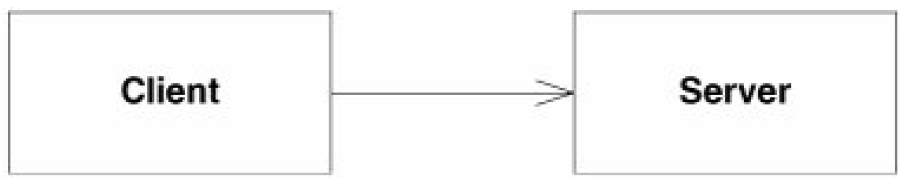
\includegraphics[width=0.7\linewidth]{figs/OCP/clientServer.PNG}
\caption{OCP brudt.}
\label{fig:clientServer}
\end{figure}


\subsubsection{Perspektiver}

\paragraph{Strategy pattern} 
En måde at opnå OCP på, kunne være brugen af et strategy pattern (eksternalisering af klasseansvar til strategier), i stedet af begynde at modificere en allerede eksisterende klasse. 

\subsection{Lisskov's Substitution Principle (LSP)}
\textit{''Subtypes must be substitutable for their base types''}\\

Hvis en Tesla er en specialisering af en bil, så bør jeg kunne bruge bilens drive() metode på teslaen.\\

Lad os sige at en base klassen bil, har en \textit{drive()} og en \textit{shiftGearUp()} metode. Teslaen kan sagtens implementere \textit{drive()} metoden men fordi det er en Tesla får vi et problem med gearskiftet! (et \textbf{throwExeption}) vil bryde OCP! Et \textcolor{green!60!black}{//Do Nothing} er sikkert fint men ikke særligt sikkert. Altså er en Tesla ikke en bil i Barbara Liskovs optik.\\

LSP handler dermed i bund og grund om ikke at bryde ”er en” kontrakten med klient koden, og altså lave et arvehieraki der opfylder en ægte specialisering.

\subsubsection{Pre -og postconditions}

\begin{enumerate}
	\item An overriding method may [only] \textbf{weaken the precondition}. This means
	that the overriding precondition should be logically "or-ed" with the
	overridden precondition.
	\item An overriding method may [only] \textbf{strengthen the postcondition}. This
	means that the overriding postcondition should be logically "and-ed" with
	the overridden postcondition.
\end{enumerate}

\subsubsection{LSP overholdt}
Hvis vi har følgende klasse Vehicle:

\begin{lstlisting}
class Vehicle {
	public void StartEngine() {
		// Default engine start functionality
	}
	public void Accelerate() {
		// Default acceleration functionality
	}
}
\end{lstlisting}

Og vi så vil aflede to klasser, Car og ElectricCar.

\begin{lstlisting}
class Car : Vehicle {
	public void StartEngine() {
		engageIgnition();
	}
	private void engageIgnition() {
		// Ignition procedure
	}
}

class ElectricCar : Vehicle {
	public void accelerate() {
		increaseVoltage();
	}
	private void increaseVoltage() {
		// Electric logic
	}
}
\end{lstlisting}

Så skal begge være lavet så de kan skiftes ud med Car klassen. Således vil følgende funktionskald ikke give fejl og stadig virke som de skal, som set fra clientens side.

\begin{lstlisting}
class Driver {
	public void Drive(Vehicle v) {
		v.StartEngine();
		v.Accelerate();
	}
}
\end{lstlisting}

\subsubsection{Brud på LSP}
Hvis vi allerede har lavet en klasse \textit{Rectangle}:

\begin{lstlisting}
class  Rectangle {
	int width, height;
	public void setHeight(int h){}
	public void getHeight(int h){}
	public void setWidth (int w){}
	public void getWidth (int w){}
}
\end{lstlisting}

Og vi så vil lave en afledt klasse \textit{Square}. Så burde dette være ligetil, men er en Square i programmering det samme som en Rectangle?

\begin{lstlisting}
class  Square : Rectangle {
	public void setHeight(int h){}
	public void setWidth (int w){}
}
\end{lstlisting}

Her vil vi få et program da højde og bredde vil blive sat til det samme. Men hvad så hvis clienten forventer føglende test kan gennemføres?

\begin{lstlisting}
class Client {
	public void AreaVerifier(Rectangle r) {
		r.setHeight(5);
		r.setWidth(4);
		
		if(r.area() != 20) {
			System.Console.WriteLine("FUCK!");
		}
	}
}
\end{lstlisting}

%\subsection{Dependency Inversion Principle (DIP)}
\subsection{Dependency Inversion Principle (DIP)}
DIP har følgende centrale punkter:\\

\textit{''High level modules should not depend on low level modules. Both should depend on abstractions.''}\\

\textit{''Abstractions should not depend upon details. Details should depend upon abstractions.''}\\

Det hedder dependency inversion fordi...\todo{hør fil 1441956 389456 og skriv hvor navnet kommer fra}
\\

Det der menes med abstraktioner her, er interfaces. Et eksempel på DIP er vores øvelse med Compressions Stocking, hvor vi fx havde nogen knapper (high-level) der kaldte noget low-level funktionalitet (blinkende LED’er osv). I stedet for at gøre knappen afhængig af low-level funktionalitetet, lader vi den afhænge af et interface.\\

Klassediagrammet kan ikke være på én side så derfor kan billedet for øvelsen kan ses på  \href{https://raw.githubusercontent.com/BjornNorgaard/I4SWD/bdd4a11a87f182d81b3ed81409a2052e45be82c3/Eksamen/Disposition/figs/compressionstockings_classdiagram.PNG}{dette billede} fra github repo'et.

\subsection{Hvordan fremmes godt SW design?}

Alle tre design principper har deres fordele og nogen, deres ulemper.

Undgå Design Smells:

\begin{itemize}
	\item Rigidity.\\
	Svært at ændre i koden, simple ændring skaber kaskader af andre lndringer.
	\item Fragility.\\
	Programmet går i stykker, ved simple ændringer.
	\item Immobility. \\
	Immobil at overføre til nyt system.
	\item Viscosity.\\
	Hacking af løsninger.
	\item Needless complexity.\\
	Siger sig selv.
	\item Needless repetition.\\
	Genbrug af kode - hellere lav en abstraktion!
	\item Opacity.\\
	Opacity er når koden er svær at forstå.
\end{itemize}

Godt software design fremmes, ved at implementere sit program, med henblik på at overholde eks. SOLID principperne. Til dette kan der specialiseres generelle løsninger (Design Patterns). Basically er keywords til godt software design: \textit{Lav kobling, høj samhørighed, stærk indkapsling Testability, Reuseabilty, Readability} osv.
\subsection{Eksempel}
Gode SOLID eksempler på \href{http://blog.gauffin.org/2012/05/11/solid-principles-with-real-world-examples/}{blog.gauffin.org}.

\subsection{Redegør for ulemper}
Alting er ikke et søm, bare fordi man har en hammer! Forkert og eller overdrevet brug af SOLID principperne, kan føre til needless complexity. Eksempelvis kan overdrevet klasseinddeling (SRP) give anledning til unødvendig kompleksitet - An axis of change is only an axis of change, if change occurs.